%!TEX root=../main.tex
\chapter{User Test Material}
\label{apdx:usertest}

\section{User Study Questionnaire}


\section{Summary of Textual Based Questions}
\paragraph*{Are there any tasks or actions that you feel cumbersome or hard to perform? Please specify if any.} \hfill 
\begin{itemize}
  \item Unclear wether to zip folders, files etc. Should instead be a small label next to the upload button, instead of link to the HowTo page. Upload should accept single or multi source file upload. Might be easier to upload from Unix systems (\textit{Count: 9}).
  \item Rerunning code is implicitly discouraged compared, and users should be notified about the behaviour (\textit{Count: 1}).
  \item Waiting a long time in the run-queue (\textit{Count: 2}).
\end{itemize}

\paragraph*{Do you feel any feedback is missing in the Climbing Mont Blanc system? Please specify.} \hfill
\begin{itemize}
  \item Feedback is good and the system clarifies the problem if there is errors (\textit{Count: 1}).
  \item Up-to-date run queue status, such as position in queue and expected queue time (\textit{Count: 11}).
  \item Little feedback during heavy system load, and show estimated progress bar instead of spinner (\textit{Count: 2}).
  \item When adding problems to your group, the ``add problem''-button should be ``grayed-out'' until a valid problem name is specified. Currently, no error message is shown when giving a invalid problem name and trying to add the problem. The same applies to the ``add member''-button on the same page (\textit{Count: 1}).
  \item ``Runtime error in small input!''-message does not give sense to untrained users (\textit{Count: 1}).
\end{itemize}

\paragraph*{Any information that is missing on the HowTo-page? Please specify.} \hfill
\begin{itemize}
  \item Contains to much text (\textit{Count: 1}).
  \item More information about run procedure, queuing multiple submissions, and possible output (\textit{Count: 1}).
  \item Exact information about format and file name conventions in uploads
\end{itemize}

\section{TDT4200 User Study Results}
There were in total 37 students completing the survey. Figures \ref{fig:oldmultiplechoice} and \ref{fig:oldmultiplechoice1} shows the results of the multiple choice questions related to CMB. Some background information about the participants is also presented in Figure \ref{fig:oldsurvey-dist}. The Figure describes the distribution amongst the year of study and area of study. A summary of the feedback given in the textual based questions and feedback received in class is found below:

\begin{itemize}
\item Feedback given from the CMB system should be improved. Both regarding compilation errors and runtime errors.
\item The format and how to structure the zip to be uploaded was unclear. Would be nice to be able to upload single source files.
\item Submission of zip files from OSX did not work.
\item The delivery zip format through ItsLearning and CMB varied, which further lead to some confusion.
\item CMB had days with long run queue time.
\item Compilation and running of code should be done in one action.
\item One should be able to delete failed submissions as a user.
\item Running the same submission one more time should result in a new submission to the high score list, not an updated entry.
\item Sometimes, submissions that were chosen to be private were shown. The bug becomes present when sorting the highscore list on one of the other metrics.
\item The login procedure requires too many clicks.
\item CMB should support command line interface instead of the User Interface to compile and run programs.
\item Submissions is not visible accessing the problem page from a group view, only when accessing the problem from the public list of problems.
\item Expected compilation time and running time should be added, and also dynamic update the highscore list when runs have completed.
\item The submissions should display the lines of code and more information about the uploaded files.
\item The sorting of the highscore list should consider energy as a secondary priority next to running time when sorting the highscore list.
\item More languages should be supported.
\item Users should be able to specify compiler flags.
\item Detect content within the uploaded zip file.
\item CMB is a really good idea; you should try to improve it.
\item It needs some improvement, but, all in all, it is a good system.
\item Overall usability is good. But the system might need some overhaul of its components.
\end{itemize}

\begin{figure}
    \centering
    \hspace*{-1.5cm}
    \begin{subfigure}[h]{0.4\textwidth}
        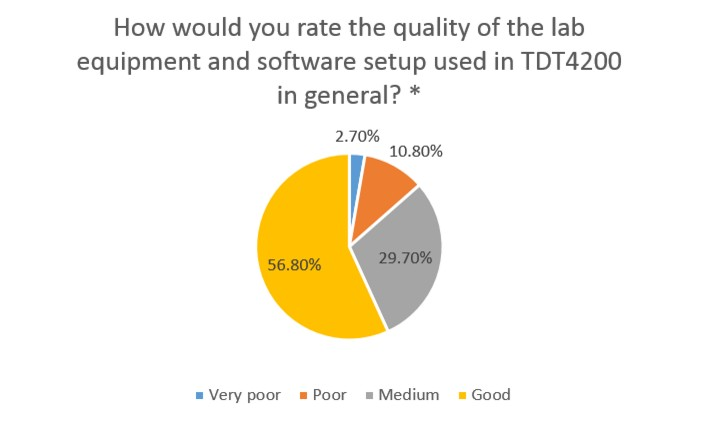
\includegraphics[width=1.5\textwidth, height=1.0\textwidth]{oldresults/equipment.jpg}
        \caption{}
        \label{fig:equipment}
    \end{subfigure}
    ~ %add desired spacing between images, e. g. ~, \quad, \qquad, \hfill etc.
      %(or a blank line to force the subfigure onto a new line)
    \hfill
    \begin{subfigure}[h]{0.4\textwidth}
        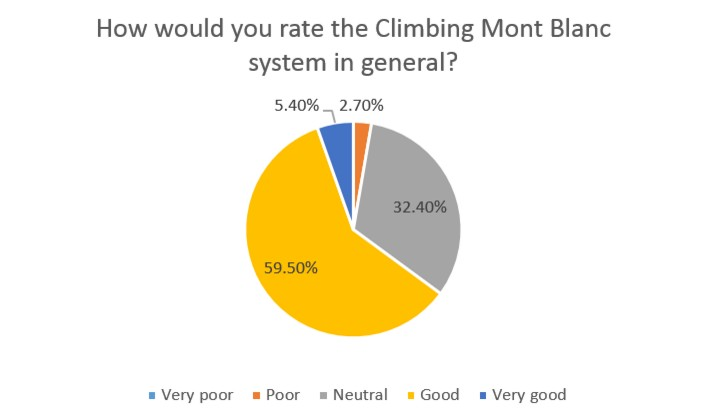
\includegraphics[width=1.5\textwidth, height=1.0\textwidth]{oldresults/cmb_general.jpg}
        \caption{}
        \label{fig:cmb-general}
    \end{subfigure}
    ~ %add desired spacing between images, e. g. ~, \quad, \qquad, \hfill etc.
    %(or a blank line to force the subfigure onto a new line)
    \hspace*{-1.5cm}
    \begin{subfigure}[h]{0.4\textwidth}
        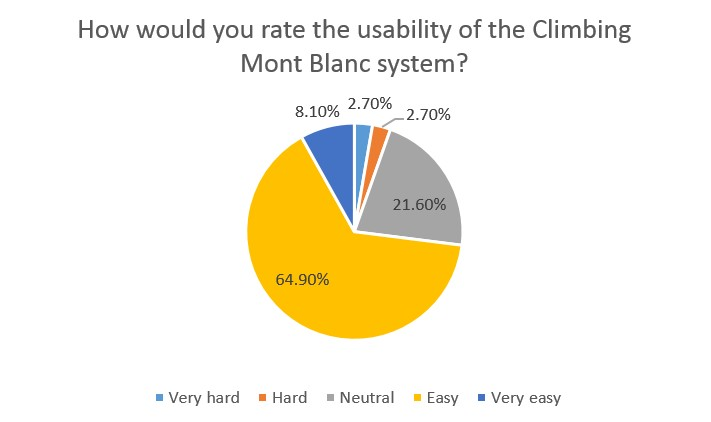
\includegraphics[width=1.5\textwidth, height=1.0\textwidth]{oldresults/cmb_usability.jpg}
        \caption{}
        \label{fig:cmb-usability}
    \end{subfigure}
    \hfill
    \begin{subfigure}[h]{0.4\textwidth}
        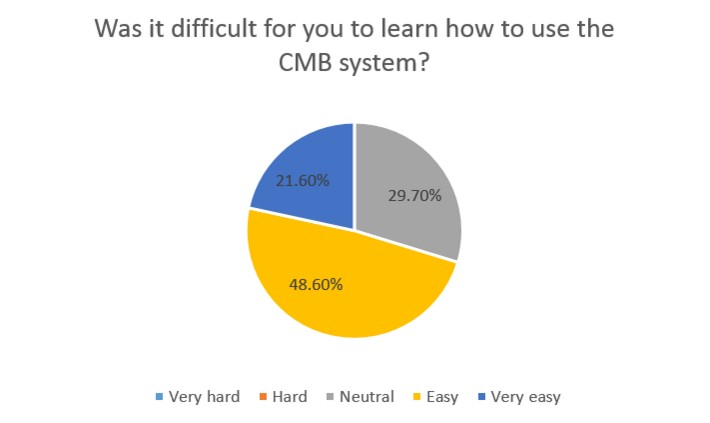
\includegraphics[width=1.5\textwidth, height=1.0\textwidth]{oldresults/cmb_learn.jpg}
        \caption{}
        \label{fig:cmb-learn}
    \end{subfigure}
    \hspace*{-1.2cm}
    \begin{subfigure}[h]{0.4\textwidth}
        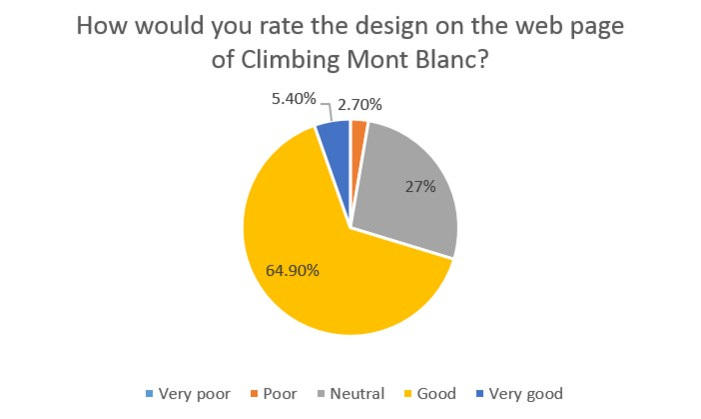
\includegraphics[width=1.5\textwidth, height=1.0\textwidth]{oldresults/cmb_design.jpg}
        \caption{}
        \label{fig:cmb-design}
    \end{subfigure}
    ~ %add desired spacing between images, e. g. ~, \quad, \qquad, \hfill etc.
      %(or a blank line to force the subfigure onto a new line)
    \hfill
    \begin{subfigure}[h]{0.4\textwidth}
        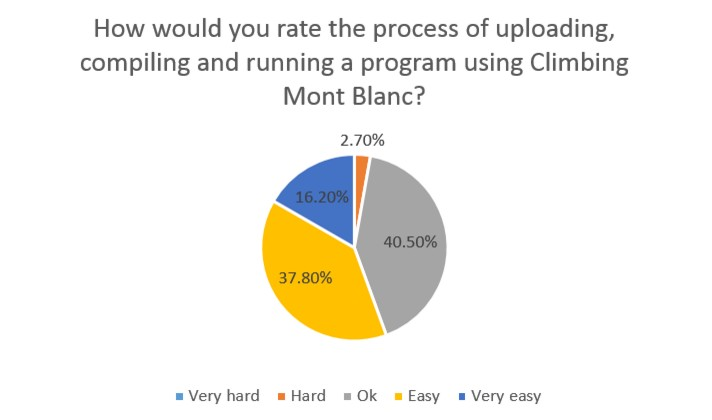
\includegraphics[width=1.5\textwidth, height=1.0\textwidth]{oldresults/cmb_tasks.jpg}
        \caption{}
        \label{fig:cmb-tasks}
    \end{subfigure}
    \caption*{CMB Related Multiple Choice Results}
    \label{fig:oldmultiplechoice}
\end{figure}

\begin{figure}
    \hspace*{-1.5cm}
    \begin{subfigure}[h]{0.4\textwidth}
        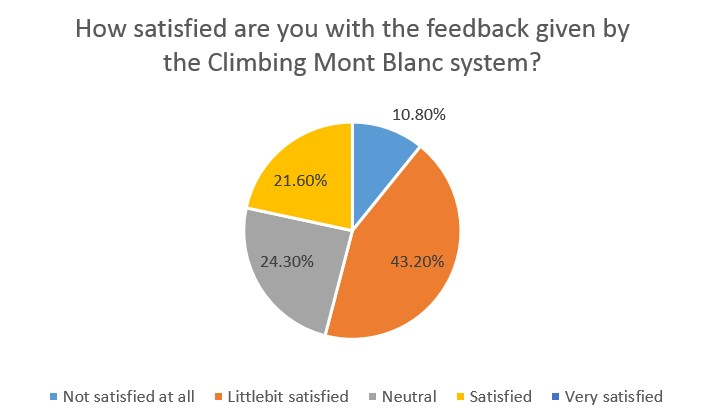
\includegraphics[width=1.5\textwidth, height=1.0\textwidth]{oldresults/cmb_feedback.jpg}
        \caption{}
        \label{fig:cmb-feedback}
    \end{subfigure}
    \hfill
    \begin{subfigure}[h]{0.4\textwidth}
        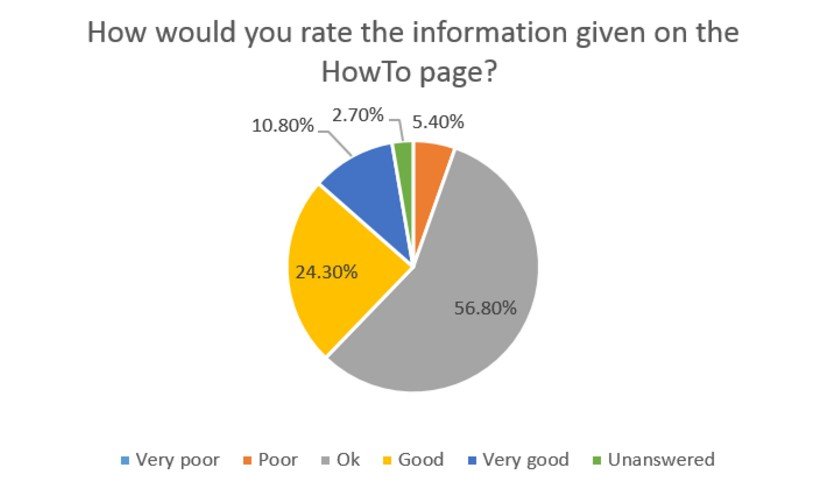
\includegraphics[width=1.5\textwidth, height=1.0\textwidth]{oldresults/cmb_howto.jpg}
        \caption{}
        \label{fig:cmb-howto}
    \end{subfigure}
    \caption*{CMB Related Multiple Choice Results (continuation of \ref{fig:oldmultiplechoice})}
    \label{fig:oldmultiplechoice1}
\end{figure}

\begin{figure}
    \hspace*{-1.5cm}
    \begin{subfigure}[h]{0.4\textwidth}
        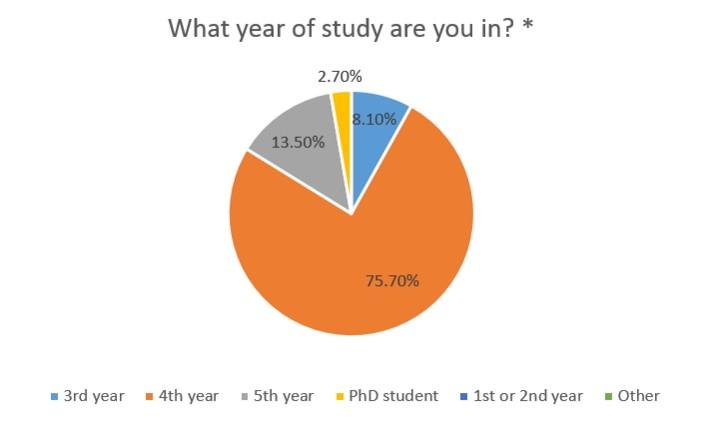
\includegraphics[width=1.5\textwidth, height=1.0\textwidth]{oldresults/participants.jpg}
        \caption{}
        \label{fig:distribution}
    \end{subfigure}
    \hfill
    \begin{subfigure}[h]{0.4\textwidth}
        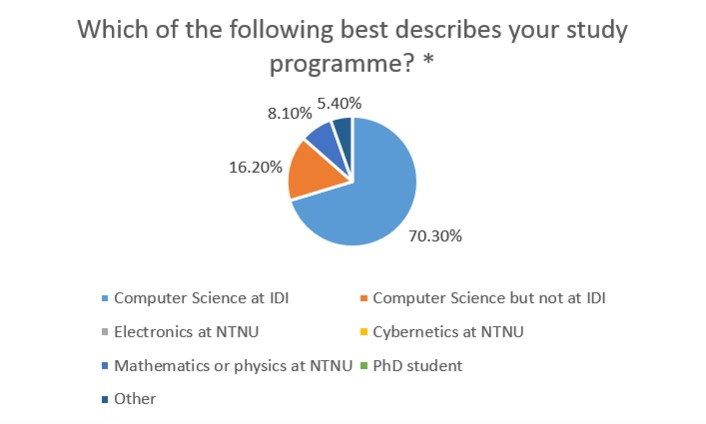
\includegraphics[width=1.5\textwidth, height=1.0\textwidth]{oldresults/distribution.jpg}
        \caption{}
        \label{fig:participants}
    \end{subfigure}
    \caption*{Participant Distribution}
    \label{fig:oldsurvey-dist}
\end{figure}
